\subsection{L’oxyde lamellaire : reférence \ce{LiCoO2}}
\label{subsubsection:oxyde_lamellaire}

\setcounter{equation}{0}
\setcounter{Q}{0}

\begin{center}
\begin{minipage}[]{0.2\textwidth}
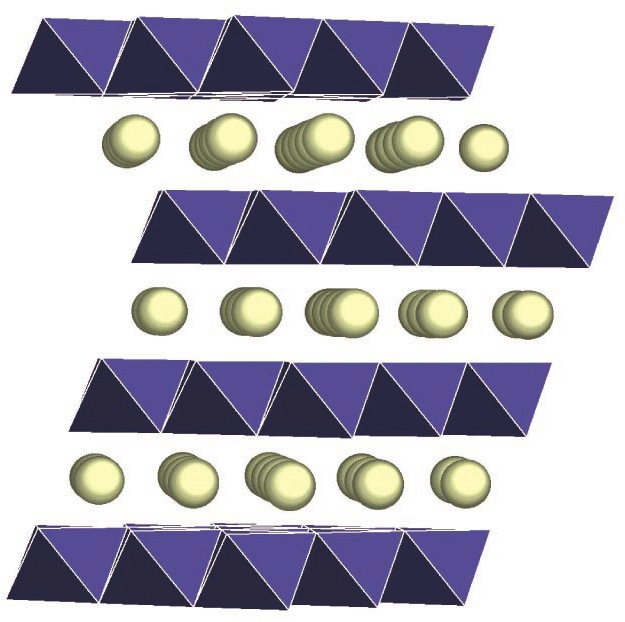
\includegraphics[height=3cm]{Ex16/Fig01c}
\end{minipage}\begin{minipage}[]{0.3\textwidth}
\captionof{figure}{Représentation de la structure sous forme de polyèdre}
\label{fig:Ex16-Fig02}
\end{minipage}
\end{center}

Comme représenté à la Fig. \ref{fig:Ex16-Fig02}, les composés lamellaires résultent d'un empilement successif :
\begin{enumerate}
\item d'octaèdres \ce{MO6}, où M est le métal participant à la "charpente" de la couche d'oxyde ;
\item d'une couche de lithium occupant des sites octaédriques, tétraédriques ou prismatiques.
\end{enumerate}

Nous allons chercher à comprendre comment visualiser ces structures en partant de vos notions élémentaires en cristallographie. Une façon de voir ces structures est de considérer une maille élémentaire où :
\begin{enumerate}
\item les métaux Li ou M occupent un réseau cubique à face centré ;
\item les oxygènes occupent tous les sites octaédriques de ce réseau.
\end{enumerate}

%Review—Li-Rich Layered Oxide Cathodes for Next-Generation Li-Ion Batteries: Chances and Challenges

\Q \label{Q:Ex16-1} Représenter la maille élémentaire CFC ainsi que les sites occupés. Indiquer le repère $(\vec{a}_c, \vec{b}_c, \vec{c}_c)$ dans ce système cubique.
\solution{Représentation du système cubique face centré en question :
\begin{center}

\includegraphics[width=0.48\textwidth]{Ex16/Corr01}
\end{center}
Les atomes d'oxygènes (resp. atomes métalliques) sont indiqués en rouge (resp. gris)
}

\Q \label{Q:Ex16-2} Identifier un axe de plans réticulaires de la maille cubique permettant de rendre compte de l'aspect lamellaire de la structure. Nommer cette série de plans.
\solution{On remarque qu'en prenant l'axe réticulaire [111], on obtient bien une succession de plans d'oxygène et de cation : 
\begin{center}

\includegraphics[width=0.35\textwidth]{Ex16/Corr02}
\end{center}
}

\Q Afin d'aboutir à une structure lamellaire à partir de la structure cubique, une projection a été proposée selon le plan définit par les vecteurs de base :

\begin{minipage}{0.48\textwidth}
\begin{align*}
\left(  \frac{\vec{a}_c + \vec{b}_c}{2} , \vec{c}_c \right)
\end{align*}
\end{minipage}\hfill \begin{minipage}{0.48\textwidth}

\includegraphics[width=\textwidth]{Ex16/Fig02}
\end{minipage}

La maille élementaire a volontairement été multipliée par 4 selon les trois axes unitaires du cube (c.-à-d. que le volume de la maille a été multiplié $\times 4^3 = 32$) . Identifier les centres métalliques qui doivent être des \ce{Li} et ceux qui doivent être des \ce{Co}. Représenter la maille élémentaire hexagonale résultante.
\solution{Un plan sur deux de cations contient des cations de lithium (gris) et l'autre des cations de cobalt (bleu).
\begin{center}
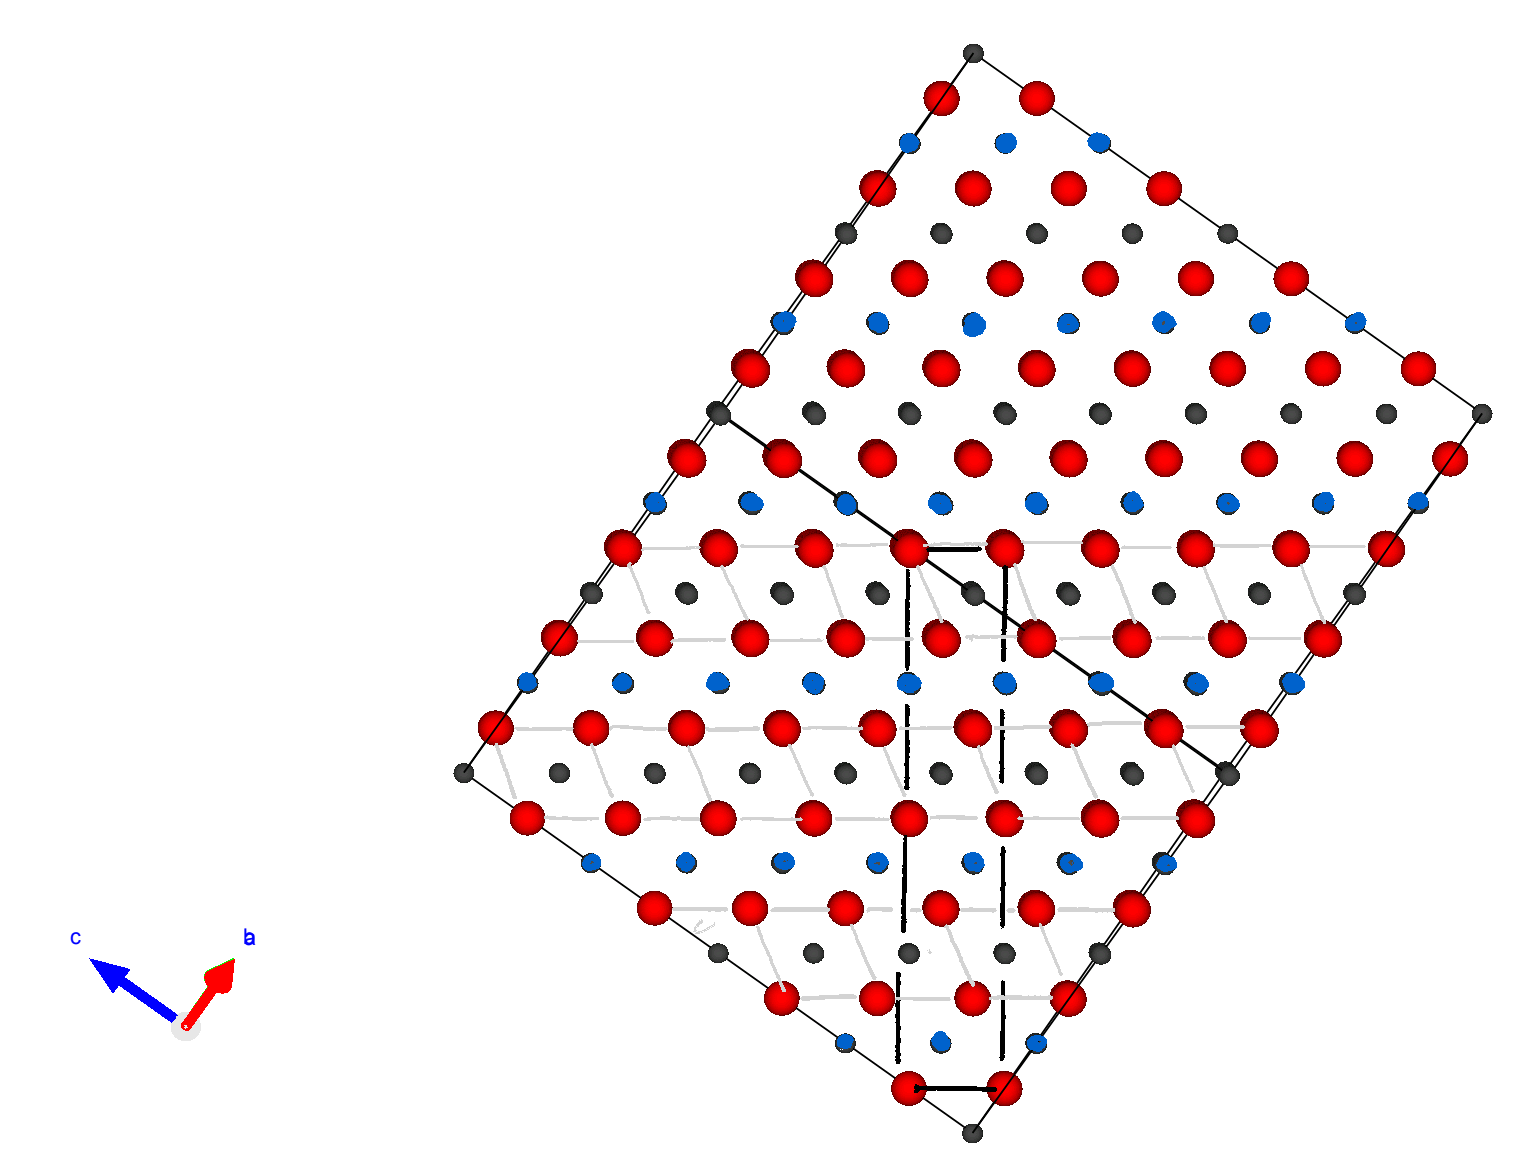
\includegraphics[width=0.35\textwidth]{Ex16/Corr03}
\end{center}
On représente la plus petite maille hexagonale résultante.
}

\begin{comment}
\Q Définir un nouveau repère $(\vec{a}_h, \vec{b}_h, \vec{c}_h)$ à partir des vecteurs de base de la Q.\ref{Q:Ex16-1}. Renommer le plan réticulaire trouvé à la Q.\ref{Q:Ex16-2} dans le système hexagonal.
\solution{
\begin{align*}
\vec{a}_h &= \\
\vec{b}_h &= \\
\vec{c}_h &= \frac{1}{\sqrt{3}}(\vec{a}_c + \vec{a}_c + \vec{a}_c)
\end{align*}
}\end{comment}


Après toutes ces constructions, la maille obtenue pour l'oxyde lamellaire \ce{LiCoO2}, matériau de la première batterie Sony (1990). Sa structure est projetée aux Fig.\ref{fig:Ex16-01a} et \ref{fig:Ex16-01b} selon les plans réticulaires (100) et (001) définis dans le nouveau repère hexagonal.

\begin{center}
\begin{minipage}[]{0.4\textwidth}
\begin{figure}[H]
\begin{centering}
\subfloat[\label{fig:Ex16-01a}]{
\includegraphics[width=2cm]{Ex16/Fig01a}}\hfill
\subfloat[\label{fig:Ex16-01b}]{
\includegraphics[height=3cm]{Ex16/Fig01b}}
\end{centering}
\end{figure}
\end{minipage}\hspace{0.5cm}\begin{minipage}[]{0.4\textwidth}
\captionof{figure}{\ref{fig:Ex16-01a} Maille conventionnelle du composé de st{\oe}chiométrie \ce{Li3Co3O6} projetée le long de (100). \ref{fig:Ex16-01b} Maille conventionnelle du composé de st{\oe}chiométrie \ce{Li3Co3O6} projetée le long de (001).}
\end{minipage}
\end{center}

\Q Nommer cette structure dans la nomenclature de Delmas. Justifier si l'interaction Li-O est plutôt de nature ionique ou covalente.
\solution{
Les atomes de lithium sont liés aux oxygènes par des octaèdres, on qualifie la structure de O. Il y a 3 plaques d'oxyde de cobalt dans la maille, on peut donc dire que la structure est \ce{O3}. Au bilan, cette variété allotropique de l'oxyde de cobalt lithié est qualifié par : 
\begin{align*}
\ce{O3-LiCoO3}
\end{align*}
\`{A} partir des données, on peut calculer la distance Li-O et calculer l'écart à l'expérience : 
\begin{center}
\begin{tabular}{ccc}
\toprule
Type de liaison & Longueur de liaison & \'{E}cart relatif \\
& \si{\pico\meter} & $\emptyset$ \\
\midrule
covalente & $134 + 66 = 200$ & $\frac{209-200}{209} \approx 0.04$\\
ionique & $128 + 76 = 204$ & $\frac{209-204}{209} \approx 0.02$\\
\bottomrule
\end{tabular}
\end{center}
où l'écart relatif est calculé comme : 
\begin{align*}
\frac{d_{Li-O}^{calc} - d_{Li-O}^{exp}}{d_{Li-O}^{exp}}
\end{align*}
De plus, en calculant de degré d'ionicité à l'aide du modèle de Pauling, on trouve : 
\begin{align*}
I = 0.78 = 78 ~ \si{\percent}
\end{align*}
\`{A} priori, ces deux arguments (surtout le second) sont en faveur d'une liaison plutôt ionique.}%O3-LiCoO3

Une autre façon de représenter la maille est d'ajouter les polyèdres de coordinations au sein de la maille. La structure cristallographique est représentée en perspective sur la Fig. \ref{fig:16-04}.

\begin{center}
\begin{minipage}[]{0.4\textwidth}
\begin{figure}[H]
\begin{centering}

\includegraphics[width=3cm]{Ex16/Fig04}
\end{centering}
\end{figure}
\end{minipage}\hspace{0.5cm}\begin{minipage}[]{0.4\textwidth}
\captionof{figure}{Polyèdres de coordination du lithium et du cobalt sur une représentation en perspective de la maille du composé de st{\oe}chiométrie \ce{Li3Co3O6}.}
\label{fig:16-04}
\end{minipage}
\end{center}


\Q Indiquer comment les octaèdres sont coordonnés entre eux.
\solution{
On a deux types d'octaèdres : \ce{CoO6} et \ce{LiO6}. Il y a donc trois coordinations possibles entre les octaèdres : 
\begin{center}
\begin{tabular}{ccc}
\hline
\ce{LiO6}-\ce{LiO6} & \ce{LiO6}-\ce{CoO6} & \ce{CoO6}-\ce{CoO6} \\
\hline
arêtes & arêtes & arêtes \\
\hline
\end{tabular}
\end{center}
}

\Q Quelle est la charge électrique des feuillets composés de polyèdres cobalt-oxygène ? 
\solution{Les ions lithium entre les feuillets sont chargés positivement. Par électroneutralité de la structure, les feuillets sont donc chargés négativement.}

\Q Cette première batterie possédait une capacité spécifique de \SI{150}{\milli\ampere\hour\per\gram} ce qui est relativement faible (on peut maintenant obtenir le double). Proposer une hypothèse expliquant cette capacité relativement faible.
\solution{Les feuillets sont chargés négativement. Une partie des ions lithium doivent nécessairement rester entre les plaques pour stabiliser la structure. Par conséquent, lors d'une charge, tous les ions lithium ne peuvent pas quitter la structure.}

\Q Comment peut-on améliorer la situation ? Pourquoi ? 
\solution{On doit stabiliser la structure cristallographique en :
\begin{itemize}
\item utilisant des cations de plus haut degré d'oxydation ; 
\item utilisant des anions plus polarisables (gros).
\end{itemize}
}

Quelques-unes de ces améliorations de la structure \ce{LiCoO2} sont étudiées en détails dans le dernier chapitre du cours.

\paragraph*{Données}
\begin{itemize}
\item Distance expérimentale \ce{Li-O} dans \ce{LiCoO2} : $d^{exp}_{Li-O} = 209 ~ \si{\pico\meter}$   
\item Rayons ioniques en \si{\pico\meter} : 
\begin{align*}
r_{Li} ( \text{IV} ) &= 59 ~ \si{\pico\meter} ; \\
r_{Li} ( \text{VI} ) &= 76 ~ \si{\pico\meter} ; \\
r_{O} &= 128 ~ \si{\pico\meter} ;
\end{align*}
\item Rayons covalents en \si{\pico\meter} : 
\begin{align*}
r_{Li} &= 134 ~ \si{\pico\meter} ; \\
r_{O} &= 66 ~ \si{\pico\meter}
\end{align*}
\item \'{E}lectronégativité de Pauling : 
\begin{align*}
\chi ( \ce{Li} ) &= 0.98 \\
\chi ( \ce{O} ) &= 3.44 \\
\end{align*}
\item Pauling est le premier à avoir défini le degré d'ionicité et a montré que dans nombre de composés ioniques \ce{A}-\ce{B}, l'ionicité de la liaison est "bien décrite" par la relation suivante : 
\begin{align*}
I = 1 - \exp \left( - \frac{( \chi (\ce{A}) - \chi (\ce{B}))^2}{4} \right)
\end{align*}
où $\chi$ est l'électronégativité du composé $A$ ou $B$ dans l'échelle de Pauling.
\end{itemize}
